\documentclass{beamer}
\usepackage[utf8x]{inputenc}
\usepackage[ngerman]{babel}	
\setbeamertemplate{navigation symbols}{}


\title{Manual JerusalemDB}
\author{Hanno Wierichs}
\institute{}
\date{\today}

 \begin{document}
	\begin{frame}[plain]
		\titlepage
	\end{frame}

	\begin{frame}{contents}
		\tableofcontents
	\end{frame} 


\section{problem} 
		\begin{frame}
			\frametitle{problem}
	example: place "House of Mary"'
					\begin{itemize}
						\item source A, 16th century: "'house of Mary, 60 double steps north the Temple Mount, not directly next to the city walls"'
						\item source B, 16th century: "'place where Mary was born, 20 double steps northwest of the lion's gate, 20 steps west of the city walls"'
						\item source C, 19th century: "'Mary's birthplace, between austrian hospice and city walls"'
					\end{itemize}					 
					\vspace{1ex}
					\begin{itemize}
						\item[$\Rightarrow$] places can have time-dependent different denominations
						\item[$\Rightarrow$] places can have time-dependent different localizations
						\item[$\Rightarrow$] places may not be always punctually located
					\end{itemize}					 					
	\end{frame}
	
	
\section{solution} 
\begin{frame}
			\frametitle{solution}
			\begin{columns}
			\column{0.6\textwidth}
			\begin{itemize}
				\item topos
					\begin{itemize}
						\item name
					\end{itemize} 
					\item place
					\begin{itemize}
						\item name
						\item located at points
						\item temporal validity 												
						\item optional: additional instances
					\end{itemize}
					\item topos $\Leftrightarrow$ place any
					\begin{itemize}
						\item optional: temporal validity for linkage
					\end{itemize}
			\end{itemize}
			\column{0.4\textwidth}
					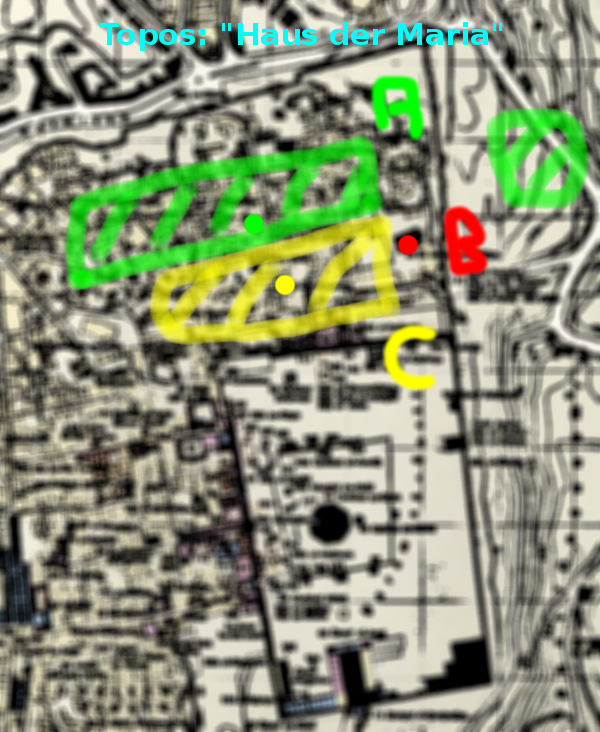
\includegraphics[width=\linewidth]{detail_1}
			\end{columns}
	\end{frame}

	\begin{frame}
			\frametitle{solution}
			\begin{itemize}
				\item one document - many entries
				\item one entry - many topos\_in\_entry
				\item topos\_in\_entry: 
				\begin{itemize}
					\item entry $\Leftrightarrow$ topos 
					\item optional: entry $\Leftrightarrow$ place 
					\item optional: alternative name for topos
					\item optional: sorting number
				\end{itemize}			 
			\end{itemize} 		
	\end{frame}

	\begin{frame}
			\frametitle{solution}
			\begin{itemize}
  					\item relational modeling:
					\begin{itemize}
						\item independent entities: author(Autor), document(Dokument), topos(Topos), place(Place)
						\item dependent entities: entry(Eintrag), topos\_in\_entry(Topos\_in\_Eintrag), placetopos(Placetopos)
					\end{itemize}
				\end{itemize} 
	\end{frame}
	
	\begin{frame}
			\frametitle{solution - modeling [schematic representation]} 
				\begin{figure}
					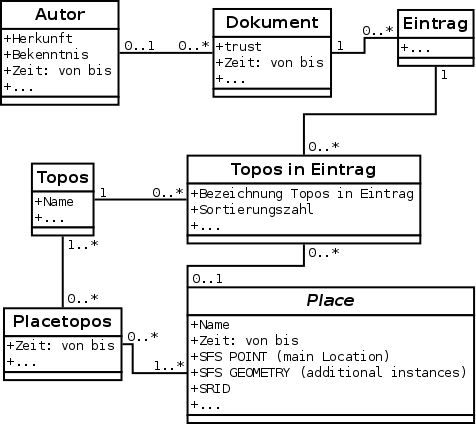
\includegraphics[scale=0.3]{detail_2.png} 
				\end{figure}			
	\end{frame}

\section{software}	
\begin{frame}
			\frametitle{software - installation} 
				\begin{itemize}
					\item JerusalemDB.jar installs required structures and serves as program entry point
					\item database directory in JerusalemData/JerusalemDB/DB
					\item[$\Rightarrow$] do not delete jar-file
					\item[$\Rightarrow$] 	do not delete or move directory JerusalemData
				\end{itemize}
	\end{frame}	

\begin{frame}
			\frametitle{software - program use - general} 
				\begin{itemize}
					\item division into table area (top left), work area (top right), map area (below)
					\item size of elements can be set by mouse; settings are persisted
				\end{itemize}
	\end{frame}	
	
\begin{frame}
			\frametitle{software - program use - menu bar} 
				\begin{itemize}
					\item traverse through history of selected records: button "'back"' respectively "'next"' (modifier key + U, modifier key + V)					
					\item show manual map interaction
					\item start analysis dialog
					\item export data (csv)
					\item exit program
				\end{itemize}
	\end{frame}		
	
	\begin{frame}
			\frametitle{software - program use - table area} 
				\begin{itemize}
					\item selection \& navigation by mouse, arrow keys or enter
					\item selection of table columns via button "'display"'
					\item selection triggers display of data in work area
					\item selection triggers display of connected data in table area
				\end{itemize}
	\end{frame}	
	
	
\begin{frame}
			\frametitle{software -  program use - work area} 
				\begin{itemize}
					\item choose work panel: hold modifier key, +T, then traverse by TAB 
					\item new record: select element "'new"' in top box
					\item selection dataset: select item in top box
					\item save: modifier key (displayed at startup)+S
					\item next dataset \& save: modifier key+N
					\item previous dataset \& save: modifier key+B
					\item reset: modifier key+Z
					\item delete: modifier key+L
				\end{itemize}
	\end{frame}	

	\begin{frame}
			\frametitle{software - program use - work area} 
				\begin{itemize}
					\item @document: integer trust value (min 1 - max 5) $\Rightarrow$ fine-grained analysis
					\item @topos\_in\_entry: sorting number $\Rightarrow$ topos\_in\_entry independent of order of entries; when selecting document, sorting numbers are displayed next to main locations
					\item @place: "'+topos"' $\Rightarrow$ associate currentyl selected place with a topos; optional: period from to
					\item @topos: "'+place"' $\Rightarrow$ associate currently selected topos with a place; optional: period from to
				\end{itemize}
	\end{frame}	


	\begin{frame}
			\frametitle{software  - program use - map area} 
				\begin{itemize}
				\item place: main location (red diamond), additional instance (green diamond)
				\item click
				\begin{itemize}
						\item if main location selected $\Rightarrow$ select place
						\item \& shift key: if place selected in table $\Rightarrow$ move main location, else $\Rightarrow$ create new place
						\item \& shift key \& ctrl key: if place selected in table $\Rightarrow$ add additional instances to place, then display added instances by shift key + click onto main location of place
\end{itemize}								
				\item confirm key actions by buttons "'save"',"'\textless"' or "'\textgreater"' [work area]
				\end{itemize}
	\end{frame}
	
	\begin{frame}
			\frametitle{software - program use - map area} 
				\begin{itemize}	
					\item click
					\begin{itemize}
							\item \& alt key: cancel selection, reload map
							\item \& shift key \& alt key: if place selected in table $\Rightarrow$ delete additional instance by clicking onto it
 							\item \& alt key \& ctrl key: display values for map adjustment
					\end{itemize}
					\item confirm key actions by buttons "'save"',"'\textless"' or "'\textgreater"' [work area] 
				\end{itemize}
	\end{frame}
	
	\begin{frame}
			\frametitle{software - program use - properties file} 
				\begin{itemize}	
					\item to be found at: JerusalemData/JerusalemResources/properties
					\item change backup interval [default: 120 min] via entry/key "'backup\_interval\_in\_minutes"'
					\item change map: modify entry/key
					\begin{itemize}
						\item defaultmap
					\end{itemize}
					\item change map: define entries/key [defaultmap as placeholder for value of entry/key "'defaultmap"']
					\begin{itemize}
						\item defaultmap\_filename
						\item map\_defaultmap\_topleftX; map\_defaultmap\_topleftY
						\item map\_defaultmap\_width; map\_defaultmap\_height
						\item map\_defaultmap\_w1; map\_defaultmap\_w2
						\item map\_defaultmap\_h1; map\_defaultmap\_h2
						\item map\_defaultmap\_x1; map\_defaultmap\_x2 
						\item map\_defaultmap\_y1; map\_defaultmap\_y2
					\end{itemize}
				\end{itemize}
	\end{frame}	
	
	\begin{frame}
			\frametitle{software - program use - properties file} 
				\begin{itemize}	
					\item change map step by step
					\begin{itemize}
						\item copy map into directory JerusalemDB/JerusalemResources/images 
						\item modify defaultmap (ex.: OSMJerusalemOldTown)
						\item define defaultmap\_filename (ex.: OSMJerusalemOldTown\_filename = OSMJerusalemOldTown.png) 
						\item define defaultmap\_absolute\_path 
						\item set size of map $\Rightarrow$ \_width \& \_height
						\item set \_w1, \_w2, \_h1, \_h2, \_x1, \_x2, \_y1, \_y2 to 1
						\item start software
						\item click on outermost upper left position on map while pressing \& alt key \& ctrl key $\Rightarrow$ \_topleftX \& \_topleftY
						\item click on upper left position on map(\_w[idth]1, \_h[eight]1) while pressing \& alt key \& ctrl key $\Rightarrow$ \_x1 \& \_y1
								\item click on lower right position on map(\_w[idth]2, \_h[eight]2) while pressing \& alt key \& ctrl key $\Rightarrow$ \_x2 \& \_y2
						\item set \_w1, \_w2, \_h1, \_h2, \_x1, \_x2, \_y1, \_y2 according to values
					\end{itemize}
				\end{itemize}
	\end{frame}		
\end{document}
